%% Figure 2: Lineage Tracking Workflow in OmicsLake
%% OmicsLake Paper - GigaScience Publication
%%
%% This figure illustrates automatic dependency tracking through dplyr pipelines.
%% Compile with: pdflatex or lualatex
%%
%% Required packages: tikz, xcolor, fontspec (for lualatex)

\documentclass[tikz,border=10pt]{standalone}
\usepackage[T1]{fontenc}
\usepackage{tikz}
\usetikzlibrary{
  shapes.geometric,
  arrows.meta,
  positioning,
  calc,
  fit,
  backgrounds,
  decorations.pathreplacing,
  calligraphy,
  shadows.blur
}
\usepackage{xcolor}

%% === GigaScience Color Palette ===
\definecolor{olBlue}{HTML}{1f77b4}      % Data tables (Parquet)
\definecolor{olGreen}{HTML}{2ca02c}     % R objects / operations
\definecolor{olOrange}{HTML}{ff7f0e}    % Parameters / refs
\definecolor{olPurple}{HTML}{9467bd}    % lake_tbl class
\definecolor{olGray}{HTML}{7f7f7f}      % Commits / metadata
\definecolor{olLightBlue}{HTML}{aec7e8} % Background
\definecolor{olLightGreen}{HTML}{98df8a}
\definecolor{olLightOrange}{HTML}{ffbb78}
\definecolor{olRed}{HTML}{d62728}       % Dependencies

%% === Node Styles ===
\tikzset{
  % Data nodes (tables in lake)
  datanode/.style={
    rectangle,
    rounded corners=4pt,
    draw=olBlue,
    fill=olBlue!10,
    line width=1.5pt,
    minimum width=2.8cm,
    minimum height=1cm,
    font=\sffamily\small\bfseries,
    text=olBlue!80!black,
    drop shadow={shadow xshift=1pt, shadow yshift=-1pt, opacity=0.3}
  },
  % dplyr operation nodes
  opnode/.style={
    rectangle,
    rounded corners=8pt,
    draw=olGreen,
    fill=olGreen!10,
    line width=1.5pt,
    minimum width=2.5cm,
    minimum height=0.9cm,
    font=\sffamily\small\bfseries,
    text=olGreen!80!black
  },
  % ref() function call
  refnode/.style={
    ellipse,
    draw=olOrange,
    fill=olOrange!10,
    line width=1.5pt,
    minimum width=2cm,
    minimum height=0.8cm,
    font=\sffamily\small\bfseries,
    text=olOrange!80!black
  },
  % lake_tbl attribute propagation
  attrnode/.style={
    rectangle,
    rounded corners=2pt,
    draw=olPurple,
    fill=olPurple!10,
    line width=1pt,
    font=\sffamily\tiny,
    text=olPurple!80!black,
    inner sep=3pt
  },
  % save_as() output
  savenode/.style={
    rectangle,
    rounded corners=4pt,
    draw=olBlue,
    fill=olBlue!20,
    line width=2pt,
    minimum width=2.8cm,
    minimum height=1cm,
    font=\sffamily\small\bfseries,
    text=olBlue!80!black,
    drop shadow={shadow xshift=1pt, shadow yshift=-1pt, opacity=0.3}
  },
  % Lineage graph node
  lineagenode/.style={
    circle,
    draw=olGray,
    fill=olGray!10,
    line width=1pt,
    minimum size=0.8cm,
    font=\sffamily\tiny\bfseries,
    text=olGray!80!black
  },
  % Data flow arrow
  dataflow/.style={
    ->,
    >=Stealth,
    line width=1.5pt,
    olBlue!70
  },
  % Pipe arrow (|>)
  pipeflow/.style={
    ->,
    >=Stealth,
    line width=2pt,
    olGreen!70
  },
  % Dependency tracking arrow
  depflow/.style={
    ->,
    >=Stealth,
    line width=1pt,
    dashed,
    olRed!70
  },
  % Attribute propagation arrow
  attrflow/.style={
    ->,
    >=Stealth,
    line width=0.8pt,
    dotted,
    olPurple
  },
  % Lineage edge
  lineageedge/.style={
    ->,
    >=Stealth,
    line width=1.2pt,
    olGray
  },
  % Step label
  steplabel/.style={
    font=\sffamily\footnotesize\itshape,
    text=olGray
  },
  % Code annotation
  codetext/.style={
    font=\ttfamily\scriptsize,
    text=black!70
  }
}

\begin{document}

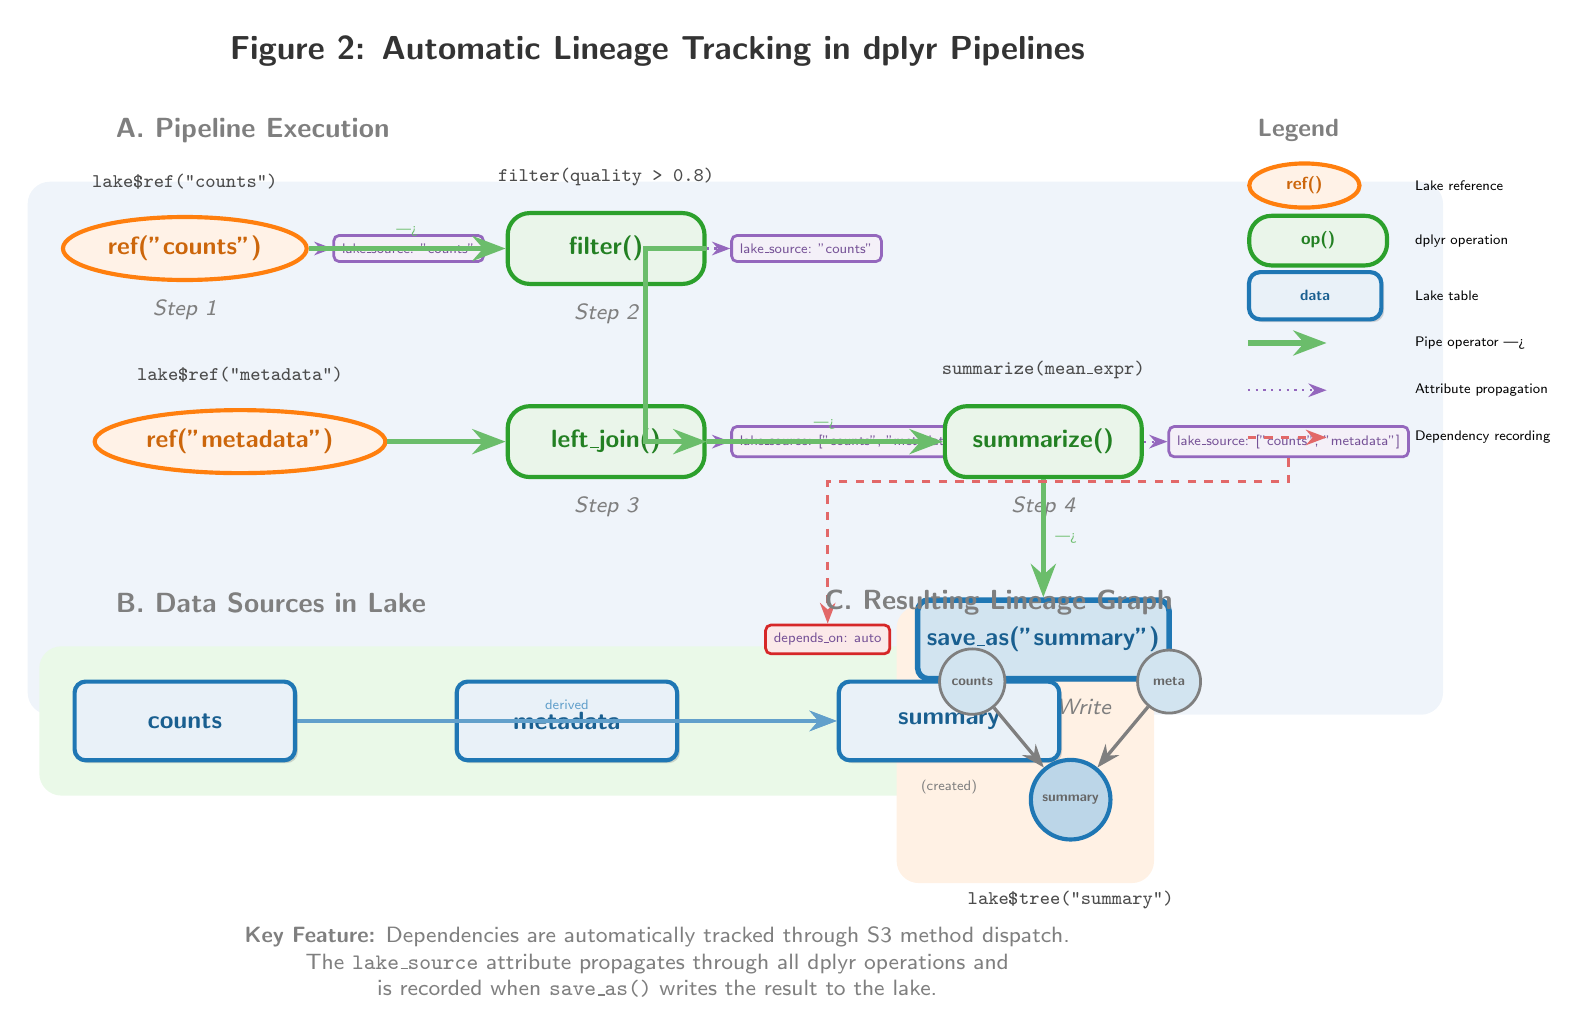
\begin{tikzpicture}[node distance=1.2cm and 1.8cm]

%% === Title ===
\node[font=\sffamily\large\bfseries, text=black!80] at (6, 7.5)
  {Figure 2: Automatic Lineage Tracking in dplyr Pipelines};

%% === Panel A: dplyr Pipeline with Dependency Tracking ===
\node[font=\sffamily\normalsize\bfseries, text=olGray, anchor=west] at (-1, 6.5) {A. Pipeline Execution};

% Step 1: ref("counts")
\node[refnode] (ref1) at (0, 5) {ref("counts")};
\node[steplabel, below=0.1cm of ref1] {Step 1};
\node[codetext, above=0.2cm of ref1] {\texttt{lake\$ref("counts")}};

% Attribute annotation for ref
\node[attrnode, right=0.3cm of ref1] (attr1) {lake\_source: "counts"};
\draw[attrflow] (ref1) -- (attr1);

% Step 2: filter()
\node[opnode, right=2.5cm of ref1] (filter) {filter()};
\node[steplabel, below=0.1cm of filter] {Step 2};
\node[codetext, above=0.2cm of filter] {\texttt{filter(quality > 0.8)}};

% Pipe arrow 1
\draw[pipeflow] (ref1) -- node[above, font=\sffamily\tiny] {|>} (filter);

% Attribute propagation
\node[attrnode, right=0.3cm of filter] (attr2) {lake\_source: "counts"};
\draw[attrflow] (filter) -- (attr2);

% Step 3: left_join() with ref("metadata")
\node[opnode, below=1.5cm of filter] (join) {left\_join()};
\node[steplabel, below=0.1cm of join] {Step 3};

% Second ref for join
\node[refnode, left=1.5cm of join] (ref2) {ref("metadata")};
\node[codetext, above=0.2cm of ref2] {\texttt{lake\$ref("metadata")}};

% Pipe arrow 2
\draw[pipeflow] (filter) -- ++(0.5, 0) |- (join);
\draw[pipeflow] (ref2) -- (join);

% Merged attribute after join
\node[attrnode, right=0.3cm of join] (attr3) {lake\_source: ["counts", "metadata"]};
\draw[attrflow] (join) -- (attr3);

% Step 4: summarize()
\node[opnode, right=3cm of join] (summarize) {summarize()};
\node[steplabel, below=0.1cm of summarize] {Step 4};
\node[codetext, above=0.2cm of summarize] {\texttt{summarize(mean\_expr)}};

% Pipe arrow 3
\draw[pipeflow] (join) -- node[above, font=\sffamily\tiny] {|>} (summarize);

% Attribute propagation
\node[attrnode, right=0.3cm of summarize] (attr4) {lake\_source: ["counts", "metadata"]};
\draw[attrflow] (summarize) -- (attr4);

% Step 5: save_as()
\node[savenode, below=1.5cm of summarize] (saveas) {save\_as("summary")};
\node[steplabel, below=0.1cm of saveas] {Step 5: Write};

% Pipe arrow 4
\draw[pipeflow] (summarize) -- node[right, font=\sffamily\tiny] {|>} (saveas);

% Dependency recording indicator
\node[attrnode, left=0.3cm of saveas, fill=olRed!10, draw=olRed] (deprec) {depends\_on: auto};
\draw[depflow] (attr4.south) -- ++(0, -0.3) -| (deprec.north);

%% === Panel B: Data Flow Visualization ===
\node[font=\sffamily\normalsize\bfseries, text=olGray, anchor=west] at (-1, 0.5) {B. Data Sources in Lake};

% Source data nodes
\node[datanode] (counts) at (0, -1) {counts};
\node[datanode, right=2cm of counts] (metadata) {metadata};

% Result node
\node[datanode, right=2cm of metadata] (summary) {summary};
\node[font=\sffamily\tiny, below=0.1cm of summary, text=olGray] {(created)};

% Data flow arrows
\draw[dataflow] (counts) -- node[above, font=\sffamily\tiny] {derived} (summary);
\draw[dataflow] (metadata) -- (summary);

%% === Panel C: Lineage Graph ===
\node[font=\sffamily\normalsize\bfseries, text=olGray, anchor=west] at (8, 0.5) {C. Resulting Lineage Graph};

% Lineage nodes
\node[lineagenode, fill=olBlue!20] (ln_counts) at (10, -0.5) {counts};
\node[lineagenode, fill=olBlue!20] (ln_meta) at (12.5, -0.5) {meta};
\node[lineagenode, fill=olBlue!30, draw=olBlue, line width=1.5pt] (ln_summary) at (11.25, -2) {summary};

% Lineage edges
\draw[lineageedge] (ln_counts) -- (ln_summary);
\draw[lineageedge] (ln_meta) -- (ln_summary);

% Lineage query annotation
\node[codetext, below=0.5cm of ln_summary] {\texttt{lake\$tree("summary")}};

%% === Legend ===
\begin{scope}[shift={(13.5, 5)}]
  \node[font=\sffamily\small\bfseries, text=olGray, anchor=west] at (0, 1.5) {Legend};

  % ref() function
  \node[refnode, scale=0.7, anchor=west] (leg1) at (0, 0.8) {ref()};
  \node[font=\sffamily\tiny, anchor=west] at (2, 0.8) {Lake reference};

  % dplyr operation
  \node[opnode, scale=0.7, anchor=west] (leg2) at (0, 0.1) {op()};
  \node[font=\sffamily\tiny, anchor=west] at (2, 0.1) {dplyr operation};

  % Data table
  \node[datanode, scale=0.6, anchor=west] (leg3) at (0, -0.6) {data};
  \node[font=\sffamily\tiny, anchor=west] at (2, -0.6) {Lake table};

  % Pipe arrow
  \draw[pipeflow] (0, -1.2) -- (1, -1.2);
  \node[font=\sffamily\tiny, anchor=west] at (2, -1.2) {Pipe operator |>};

  % Attribute flow
  \draw[attrflow] (0, -1.8) -- (1, -1.8);
  \node[font=\sffamily\tiny, anchor=west] at (2, -1.8) {Attribute propagation};

  % Dependency edge
  \draw[depflow] (0, -2.4) -- (1, -2.4);
  \node[font=\sffamily\tiny, anchor=west] at (2, -2.4) {Dependency recording};
\end{scope}

%% === Background boxes for panels ===
\begin{scope}[on background layer]
  % Panel A background
  \node[fit=(ref1)(saveas)(attr4), inner sep=12pt,
        fill=olLightBlue!20, rounded corners=8pt] {};

  % Panel B background
  \node[fit=(counts)(summary), inner sep=12pt,
        fill=olLightGreen!20, rounded corners=8pt] {};

  % Panel C background
  \node[fit=(ln_counts)(ln_summary), inner sep=15pt,
        fill=olLightOrange!20, rounded corners=8pt] {};
\end{scope}

%% === Key Insight Annotation ===
\node[font=\sffamily\footnotesize, text=olGray, align=center, anchor=north] at (6, -3.5) {
  \textbf{Key Feature:} Dependencies are automatically tracked through S3 method dispatch.\\
  The \texttt{lake\_source} attribute propagates through all dplyr operations and\\
  is recorded when \texttt{save\_as()} writes the result to the lake.
};

\end{tikzpicture}

\end{document}
